\section{Classification}

\subsection{Introduction (*)}
Entriamo un po' più nella componente di validazione nei modelli di classificazione supervisionata.
La cosa più importante è \textbf{capire cosa stiamo facendo} in quanto quando sia applicano algoritmi di machine learning è facile perdersi.

Nel solito dataset vogliamo determinare se un cliente abbandonerà o meno il nostro servizio, per farlo cerchiamo di utilizzare una particolare combinazione di attributi. Bisogna innanzitutto vedere di che tipo siano le variabili presenti nel nostro database.

Dobbiamo essere in grado sia di prevederlo che di capire \textbf{perché} qualcuno ha abbandonato. Svolgiamo questo compito con un modello di \textbf{classificazione}. Un modello di classificazione è un modello che sfrutta alcuni attributi del dataset (\textbf{attributi esplicativi}) per prevedere un valore di un altro attributo (\textbf{attributo di classe}).

\begin{figure}[H]
	\hspace{-0.5cm}
	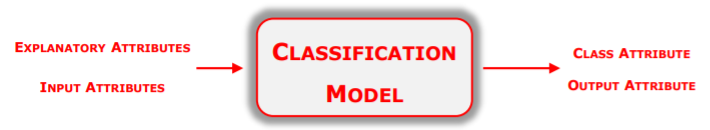
\includegraphics[height=0.2 \linewidth]{classification/pict/class_model.png}
	\caption{processo di classificazione}
\end{figure}

\begin{defn}
	Le variabili in input si chiamano \textbf{variabili esplicative}.
\end{defn}

\begin{defn}
	Le variabili in output si chiamano \textbf{variabili di classe}.
\end{defn}

\begin{defn}
	 Un \textbf{modello di classificazione} è qualcosa che risolve un problema di classificazione:
	\begin{itemize}
		\item \textbf{Modello descrittivo}: serve come strumento di spiegazione per distinguere tra oggetti di classi diverse
		\item \textbf{Modello predittivo}: predice la classe di un record sconosciuto, pu\`o essere visto come una \underline{scatola nera} che asssegna una label di una classe al record sconosciuto
	\end{itemize}
\end{defn}

\begin{defn}
	La tecnica di classificazione o \textbf{classificatore} è un approccio sistematico per costruire un modello di classificazione su un dataset.
\end{defn}
Il classificatore segue il seguente processo:

\begin{figure}[H]
	\centering
	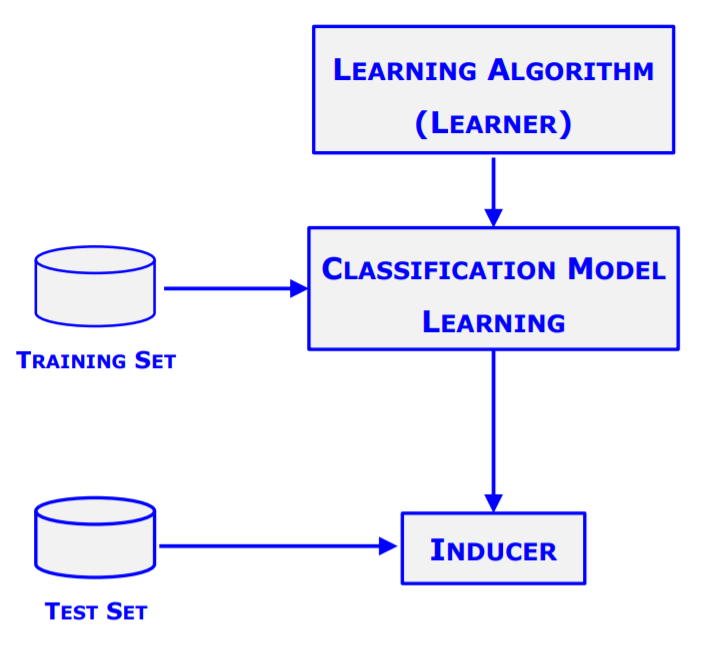
\includegraphics[height=0.6 \linewidth]{classification/pict/class_process.png}
	\caption{processo di creazione della classificazione}
\end{figure}

\begin{defn}
	Il \textbf{training set} consiste in dei record in cui tutti i valori degli attributi sono noti.
\end{defn}.  

\begin{defn}
	Il \textbf{test set} consiste in dei record i cui valori dell'attributo di classe sono sconosciuti (o presunti tali).
\end{defn}

Si utilizza quindi un algorimo di learning (\textbf{Learner}) sul training set, passaggio definito come \textbf{Classification Model Learning}. 

\begin{defn}
	L'output di questa operazione è un'istanza del modello di classificazione chiamato \textbf{Inducer}. All'inducer è chiesto di predire il valore della classe attributo per il test set. 
\end{defn}

La chiave di tutto è la scelta dell'algoritmo learner per l'apprendimento. Inoltre la scelta degli attributi esplicativi è fondamentale, infatti alcuni di essi possono essere solo ridondanti nel processo e generare solo rumore. Tramite l'analisi delle performace si possono valutare queste due scelte. 

Bisogna valutare ora le performance del modello inducer. Uno dei modi per analizzare se è efficace è la \textbf{matrice di confusione}. 

Nelle righe vi sono i veri valori delle classi, nelle colonne i valori predetti dall'inducer. Il numero di righe è uguale al numero di colonne e corrispondono al numero di classi da predire.

\begin{figure}[H]
	\centering
	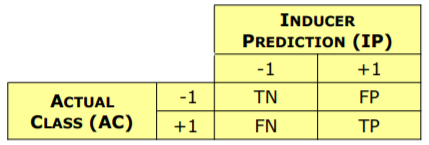
\includegraphics[height=0.25 \linewidth]{classification/pict/matrconf.png}
	\caption{modello di matrice di confusione}
\end{figure}
All'interno sono identificati i risultati dei test e sono così classificati:
\begin{itemize}
	\item \textbf{TN - vero negativo}: num. di record dove AC=-1  che sono stati corretamente predetti IP=-1
	\item \textbf{FN - falso negativo}: num. di record dove AC=+1  che sono stati erroneamente predetti IP=-1
	\item \textbf{TP - vero positivo}: num. di record dove AC=+1  che sono stati corretamente predetti IP=+1
	\item \textbf{FP - falso positivo}: num. di record dove AC=-1  che sono stati erroneamente predetti IP=+1
\end{itemize}

\begin{defn}
	La misura più utilizzata come metrica di performance è l'\textbf{accuratezza}:
	
	\[accuracy = \frac{\sum_{i = 1}^{n} diagonal}{\sum_{i=1}^{n}elements} = \frac{\#CorrPrediction}{\#Prediction} = \frac{TN + TP}{TN + TP + FN + FP}\] 
	
	La misura complementare che troveremo indicata è quella degli elementi:
	
	\[error = \frac{FN + FP}{TN + FN + FP + TP} =  1 - accuracy\]
\end{defn}

\subsection{Tecniche di classificazione}

Una tecnica di classificazione è un modo sistematico di aggredire un dataset e costruire i modelli di classificazione, in particolare possiamo dividerle in 4 macro categorie:
\begin{itemize}
	\item \textbf{Euristiche}: ispezionano il suo vicinato come (Decision Trees, Random Forest, Nearest Neighboor)
	\item \textbf{Regression Based}: usa la probabilità condizionata parametrica, es regressione logica
	\item \textbf{Separazione}: partiziona lo spazio degli attributi, fa riferimento alle Support Vector Machine e alle Artificial Neural Network
	\item \textbf{Probabilistici}: usano la formula di Bayes (Naive Bayes ecc...).
\end{itemize}

Forniremo una overview di tutte queste, non le tratteremo nel dettaglio, partiamo da quelli \textbf{Euristici}.

\subsubsection{Decision Tree}
I modelli decision tree sono bodelli basati euristici. 

Un \textbf{albero di decisione} ha innanzitutto una rappresentazione grafica precisa. Vi sono 2 elementi: nodi e archi. Il \textbf{nodo} rappresenta un sottoinsieme del dataset, gli \textbf{archi} sono usati per modellare gli output di modelli diversi di dataset.

\begin{figure}[H]
	\centering
	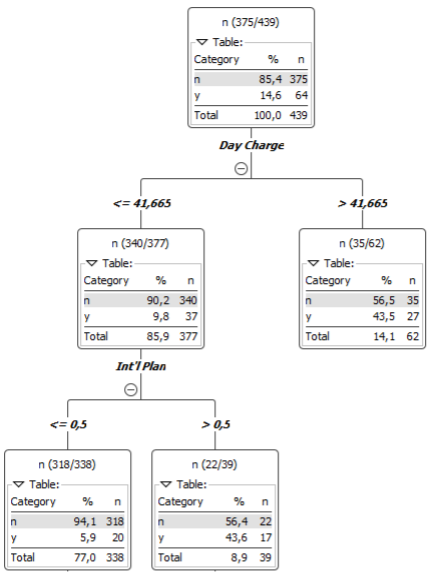
\includegraphics[height=0.7 \linewidth]{classification/pict/decision_tree.png}
	\caption{modello decision tree}
\end{figure}

I suoi ingredienti pricnipali sono:
\begin{itemize}
	\item \textbf{Root node} (nodo radice): non ha archi in ingresso ma può averne più di due in uscita
	\item \textbf{Internal nodes} (nodi interni): hanno un solo arco in ingresso e alemeno due in uscita
	\item \textbf{Leaf} (nodi foglia o terminali): sono nodi interni senza archi in uscita e con esattamente un arco in ingresso.
\end{itemize}

Cerchiamo di capire come si forma questo albero: ad ogni nodo è associato un determinato schema.

Ogni record viene classificato partendo \textbf{dall'alto} (radice) fino \textbf{al basso} (nodi foglia).

Leggo il primo nodo (radice) abbiamo l'indicazione di un attributo: nell'esempio se 'day charge' sia $\le 41,665$ o  $>$ e dividere l'albero in due nodi. Se la risposta è vera allora mi muovo in un nodo altrimenti nell'altro. All'interno del nuovo nodo ho di nuovo la valutazione di una variabile, e proseguo cos\`i finch\`e raggiungo un nodo foglia.
Quando arriviamo ad una foglia devo fornire una risposta, ovvero conto la classe più frequente ed rispondo al chiamante con essa (es. churn = n).

Il decision tree può essere usato per attributi nominali, ordinali così come intervalli numerici e coefficienti.
 
Diverse misure possono essere usate per selezionare la politica di node splitting ottima: \textit{entropia}, \textit{indice di Gini} e il \textit{classification error}. Esso comunque dipende anche dal tipo di attributo: \textit{binario}, \textit{nominale} e \textit{continuo}. 

E' un modello che risponde sempre \textit{la classe più frequente} ed è un modello praticamente inutile quando ho delle classi particolarmente sbilanciate. Sono evidentemente test univariati, ciò che faccio è costruire iper parallelepipedi del nostro dataset. Vanno a definirsi delle rette per il cambio di classificazione: \textbf{decision boundary}.

\begin{figure}[H]
	\centering
	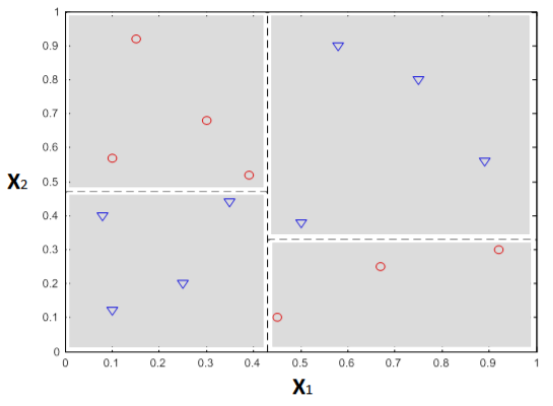
\includegraphics[height=0.5 \linewidth]{classification/pict/decision_boundary.png}
	\caption{decision boundary}
\end{figure}

Il risultato di queste rette fa la differenza sulla capacità di evidenziare dove ci siano elementi di una certa classe, devo quindi imparare a posizionare questi iperpiani: \textbf{Voglio partizionare il mio spazio in iperpiani massimizzando l'accuratezza.}

Non c'è alcuna ragione per cui io non possa usare degli splitting multipli e non solo su binari, posso farlo anche su valori nominali.

\subsubsection{Regressione Logistica Binomiale}
La regressione logistica è un metodo di classificazione basato sulla regressione.

Assumiamo che la variabile di classe Y sia compresa tra $\{0,1\}$, allora la regressione logistica binaria calcola a posteriori la probabilità che Y dia il valore dell'input ovvero le variabili esplicative 
Servono per risolvere problemi di regressione binaria a diversi livelli. E' applicabile ad attributi continui e con certe accuratezze anche ad attributi nominali.

Si assume l'attributo di classe $Y = \{0,1\}$, allora il classificatore a regressione logistica binomiale calcola a posteriore la probabilit\`a che $Y$ assuma il valore di un input esplicativo \underline{$X$}. Si cacola come segue:

\[P(Y = 0 | \underline{X}= \underline{x}) = \frac{1}{1+exp(\underline{x} \cdot \underline{w})}\]

\[P(Y = 1 | \underline{X}= \underline{x}) = \frac{exp(\underline{w} \cdot \underline{x})}{1+exp(\underline{w} \cdot \underline{x})}\]

dove $\underline{w}$ \`e chiamato il vettore parametro.

\begin{figure}[H]
	\centering
	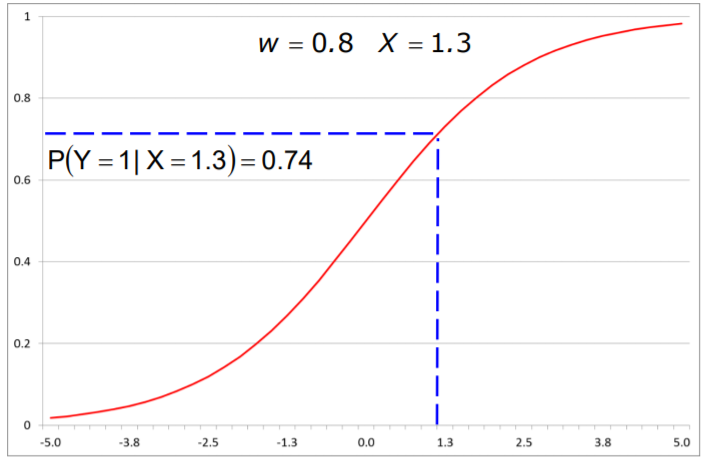
\includegraphics[height=0.5 \linewidth]{classification/pict/regr_logistic.png}
	\caption{regressione logistica}
\end{figure}

In questo modo vengono portate le probabilità di appartenere ad una certa classe.	

Vi sono poi diversi modelli derivati dal decision tree, come il Random Forest.
 
\textbf{Random forest}: \`e un comitato di alberi di decisione. Sostanzialmente usa degli attributi che sono in generale sottoinsiemi degli attributi, ogni albero può avere un sottoinsieme differente di attributi. Ogni albero usa attributi in modo randomico. Ogni albero apprende a modo suo e il random forest in base a dei parametri (regione dello spazio) decide a quale albero ascoltare per la decisione. 

\subsubsection{Support Vector Machines}
La tecnica Support Vector Machines è un metodo di classificazione con separazione. Lo scopo \`e separare o "apprendere" classi che vogliamo classificare. 

Consideriamo uno spazio bidimensionale in cui sono rappresentati $m$ record dove due attributi continui vengono misurati: $D = \{(\underline{x}_1, y_1),...,(\underline{x}_m, y_m)\}$ dove $\underline{x}_i \in R^2$ e $y_i \in \{-1, +1\}$

L'idea è quella di tracciare una retta (se ho due sole classi) per cui definisco l'area di appartenenza di una o dell'altra classe. 

\begin{figure}[H]
	\centering
	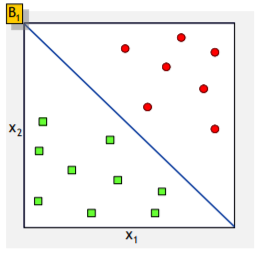
\includegraphics[height=0.4 \linewidth]{classification/pict/svm.png}
	\caption{support vector machine - una possibile retta}
\end{figure}

La retta in questione è definita dalla seguente equazione:

\[\underline{w} \cdot \underline{x} + b = w_1 x_1 + w_2 x_2 + b = 0\]

per orientare la retta utiliziamo il vettore $\underline{w} = [w_1,w_2]$ oppure $b$. ($\underline{w}$ fa ruotare, $b$ fa traslare)\\
se la retta esiste allora l'insieme delle istanze è \textit{linearmente separabile}.

\textit{Problema}: vi sono pi\`u (anche infinite) rette utilizzabili per effettuare la separazione, quale devo scegliere? Perch\`e non basta trovare una retta che funziona, ma la retta migliore per quando si dovr\`a valutare dati nuovi. Si crea una sorta di area grigia nella quale non so dire esattamente quale delle due classi categorizzare (\textbf{Linear Decision Boundary}).

\begin{figure}[H]
	\centering
	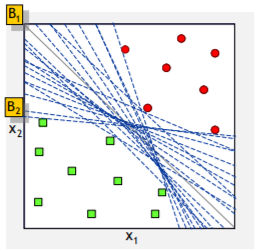
\includegraphics[height=0.4 \linewidth]{classification/pict/svm_rette.png}
	\caption{support vector machine - tante possibili rette}
\end{figure}

Devo sostanzialmente trovare una retta che \textbf{massimizza il margine di errore}, l'\textit{optimal linear decision boundary}. 

\begin{figure}[H]
	\hspace{-0.5cm}
	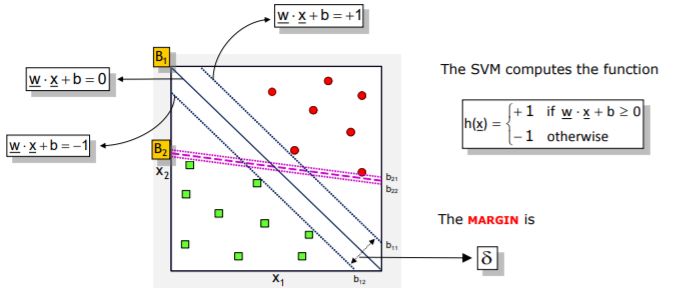
\includegraphics[height=0.45 \linewidth]{classification/pict/svm_boundary.png}
	\caption{support vector machine - boundary}
\end{figure}

la retta $B_1$ è nettamente preferita rispetto alla retta $B_2$ in quanto ha un margine di supporto $\delta$ maggiore. 

Naturalmente per n attributi bisogna trovare l'iperpiano ottimale per dividere un determinato insieme di istanze. Matematicamente parlando si cerca di massimizzare il margine $\delta = 1 / |w|^2$, la retta ha la seguente impostazione: $\bar{w} \cdot \bar{x} + b = 0$, le rette ai confini del margine sono fissate a $\bar{w} \cdot \bar{x} + b = 1$ e $\bar{w} \cdot \bar{x} + b = -1$. 

L'argomento della retta \`e in 2 dimensioni, per\`o dopo aver applicato la funzione $h(\underline{x})$ quella retta diventa un piano che va a $-1$ da un lato e a $+1$ dall'altro.

Il training di una \textbf{SVM Linear Hard-margin} formulando e risolvendo il seguente problema matematico: 

\[ \min_{\underline{w},b} \frac{1}{2}\underline{w} \cdot \underline{w}^T \]
\qquad s.t.
\[ y_i (\underline{w} \cdot \underline{x}_i + b) \ge 1 \quad \forall i = 1, ..., m\]

È un problema di programmazione quadratica con vincoli lineari i quali devono essere risolti con tecniche numeriche speciali.

Per trovare la retta devo minimizzare l'inverso del margine $\delta$\\
bisogna imporvi dei vincoli per ogni attributo, se $\underline{w}$ e $\underline{x}$ sono \textit{concordi in segno} (positivo o negativo) allora classifica perfettamente perch\`e il risultato è $>= 1$. Garantiscono che tutti i casi del dataset siano classificati correttamente e tra tutti i casi che classificano correttamente scelgo quello che massimizza il margine. 

Non risolveremo questa formula di ottimizzazione in modo diretto, ma la sua formulazione \textbf{duale}. In ogni caso questa formulazione funziona bene se il problema \`e \underline{linearmente separabile}.

Nei casi \textbf{non} linearmente separabili, non esiste \textbf{mai} una retta in grado di separare correttamente le classi. In questi casi la formulazione precedente non ammette soluzione, perch\'e per alcuni dati i vincoli non ammettono soluzione. 

Si introduce allora la \textbf{Linear Soft-margin}:

\[ \min_{\underline{w},b,\underline{\epsilon}} \frac{1}{2}\underline{w} \cdot \underline{w}^T + \Delta \sum_{i=1}^{m} \epsilon_i \]
\qquad s.t.
\[\forall_{i=1}^m :  y_i (\underline{w} \cdot \underline{x}_i + b) \ge 1 - \epsilon \] \[\forall_{i=1}^m : \epsilon \ge 0\]

le $\epsilon$ devono essere non negative (variabili di slack), se utilizzo questo parametro di una certa quantit\`a per ammettere un errore allora esiste almeno una retta che risolve il problema di ottimizzazione. Ho sostanzialmente \textit{rilassato} il problema di ottimizzazione, in particolare i vincoli. Graficamente parlando \`e come traslare degli elementi di una classe diversa dalla regione di appartenenza verso la regione della classe di quell'elemento.

\textbf{NB}: i vettori di supporto sono quelle osservazioni che sono sul bordo del margine

\textbf{Problema}: se la separazione deve avvenire con una funzione \textbf{non lineare}.
 
\textbf{Soluzione}: Si va a cercare una trasformazione che porti dallo spazio originale in uno spazio delle features in cui posso applicare una separazione lineare. Nel nuovo spazio sono in grado di separare il nuovo dataset in due diverse classi (vedi immagine che segue). 

\begin{figure}[H]
	\hspace{-0.5cm}
	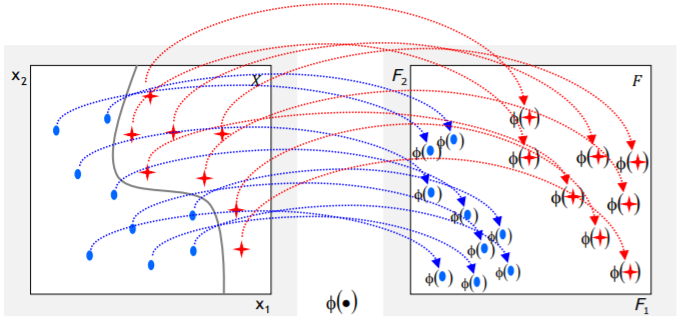
\includegraphics[height=0.45 \linewidth]{classification/pict/svm_nonlinear.png}
	\caption{support vector machine - non lineare}
\end{figure}

In questo modo posso sfruttare tutta la metodologia precedente ma in uno spazio "controllato". Bisogna trovare però una trasformazione $\phi()$ che mappi X in F.

La nuova Linear Deision Boundary nello spazio delle feature F è definito dalla seguente equazione: $\phi$: $underline{w} \cdot \phi(\underline{x}) + b = 0$. 

Il modello diventa:

\[ \min_{\underline{w},b} \frac{1}{2}\underline{w} \cdot \underline{w}^T \]
\qquad s.t.
\[ y_i (\underline{w} \cdot \phi(\underline{x}_i) + b) \ge 1 \quad \forall i = 1, ..., m\]

per l'algoritmo di apprendimento utilizziamo sostanzialmente delle funzioni kernel: $K(\underline{u}, \underline{v}) = \phi(\underline{u}) \cdot \phi(\underline{v})$. Queste funzioni kernel sono delle funzioni di similarit\`a calcolate nello spazio attributi originale di $x$ e sono riferite alla funzione kernel.

\subsubsection{Multi-Layer Perceptron o Artificial Neural Network}
Il Multi-Layer Perceptron (MLP) è una tecnica di classificazione che si basa sulla separazione dello spazio degli attributi. Oggi si utilizzano molto per il deep learning.
\begin{defn}
	Un modello \textbf{MLP Multi-Layer Perceptron} consiste in neuroni artificiali che comunicano in modo unidirezionale, dall'input X alla variabile di classe (volendo ci possono essere pi\`u neuroni di ouput).
\end{defn}

\begin{figure}[H]
	\hspace{-0.5cm}
	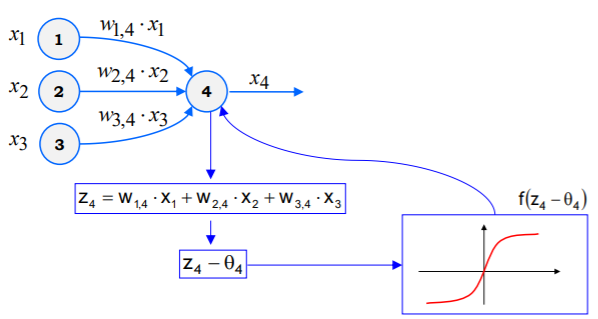
\includegraphics[height=0.45 \linewidth]{classification/pict/mlp.png}
	\caption{modello MLP}
\end{figure}

In figura vi sono 3 neuroni di parametri continui, viene aggiunto un quarto neurone che calcola una funzione. Ogni input nel neurone ha associato in peso $w$.
Il neurone calcola una \textbf{combinazione lineare} tra gli input ed il peso dato ad esso, il j-esimo neurone calcola: 

\[ y_j = f(\sum_{i=1}^{n} w_{i,j} \cdot x_i - \theta_j)\] 

Ad esempio il quarto neurone in figura:  $z_4 = w_{1,4} \cdot x_1 + w_{2,4} \cdot x_2 +w_{3,4} \cdot x_3$.
A questo calcolo viene posto una soglia threshold di valore
$\theta$ applicato alla combinazione lineare. Successivamente il neurone risponde con un valore pari all'applicazione di una funzione di attivazione rispetto all'input meno il threshold, 
nel nostro caso $f(z_4-\theta_4)$. 

\begin{defn}
	In ciascun neurone viene quindi definita la \textbf{funzione di attivazione (o trasferimento)} che restituisce il valore che lui trasferir\`a ad un altro neurone o strato con cui comunica. 
\end{defn}Storicamente le funzioni applicazione sono la tangente iperbolica e la funzione logistica (intervallo tra -1 e 1 e tra 0 e 1). Oggi vengono utilizzate delle funzioni non derivabili pi\`u complesse, come funzioni \textbf{RELU} (Retify Linear Unit) che assumono valore 0 nel semiasse negativo e 1 nel semiasse positivo.
\\

Vi sono 3 tipi di neuroni: di input, di output e nascosti:
\begin{itemize}
	\item \textbf{input} sono collegati con le variabili esplicative e con \textit{ciascun} nodo nascosto
	\item \textbf{nascosti} (o hidden) ricevono i segnali dai neuroni di input e il segnale viene propagato a quelli di ouput
	\item \textbf{output} sono associati alla variabile di classe e ricevono i segnali da visualizzare
\end{itemize}

Ogni neurone di input \`e connesso con ogni neuroni di strato nascosto  ed ogni nodo di strato nascosto comunica con il nodo di output, rete \textbf{fully-connected}. Ogni arco ha associato un peso e ogni nodo ha un valore di soglia $\theta_j$ e una funzione di attivazione. 

\begin{figure}[H]
	\centering
	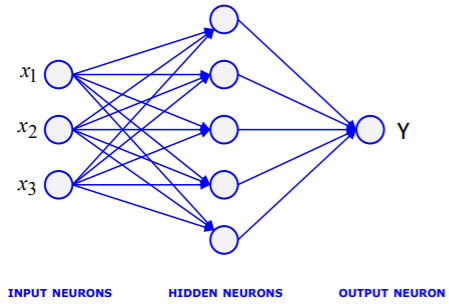
\includegraphics[height=0.5 \linewidth]{classification/pict/mlp_struct.png}
	\caption{modello MLP semplice}
\end{figure}

Per la disposizione dell'architettura ho diverse scelte da fare: quanti neuroni usare, quanti nello strato nascosto, quanti strati nascosti usiamo, che funzione di attivazione, ecc.

Determinare l'architettura della nostra rete è fondamentale per avere buone performance. Posso pensare di aggiungere un \textbf{livello} di neuroni nascosti. Non vi sono vincoli rispetto a comunicare saltando livelli. \textbf{Non} si pu\`o per\`o comunicare all'indietro, infatti queste reti sono chiamate \textbf{feed-forward neural network} (possono possedere fino a centinaia di strati nascosti).

\begin{figure}[H]
	\centering
	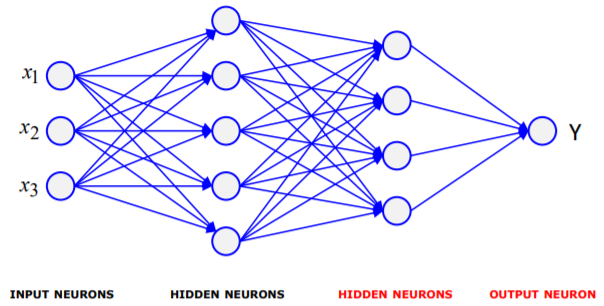
\includegraphics[height=0.5 \linewidth]{classification/pict/mlp_esempio.png}
	\caption{esempio MPL con 2 strati nascosti}
\end{figure}

Per migliorare l'apprendimento si pu\`o propagare le valutazioni fatte all'output per tutti i nodi risalendo fino all'input. Modificando i pesi degli archi. Questa cosa funziona bene e ha senso con le RELU.

Il problema MLP. non ha soluzione oggi, pertanto si procede in modo \textbf{empirico}, non \`e ancora possibile arrivare ad una soluzione ottima, non si riesce a capire se si ha raggiunto il massimo/minimo globale ma si cerca quella che dà risultati accettabili e migliori di altri. Numero di nodi, archi o livelli nascosti scelto in base all'esperienza.

\textbf{NB}: classificare non significa saper approssimare!! soprattutto per i modelli basati sulla separazione dello spazio delle feautures.

\subsubsection{Classificatori bayesiani}
I \textbf{classificatori probabilistici} calcolano la probabilit\`a condizionata secondo il \textbf{teorema di Bayes} e cercano di capire il valore della classe attributo dalle altre variabili. 

\begin{defn}

La \textbf{formula di Bayes} calcola la probabilità che un evento accada dati altri eventi: 

\[P(Y|\underline{X}) = \frac{P(\underline{X}|Y) \cdot P(Y)}{P(\underline{X})}\]

dove:
\begin{itemize}
	\item $P(Y)$ è la probabilit\`a della classe attributo
	\item $P(\underline{X}|Y)$ la verosimiglianza di un vettore di attributi data la classe attributo
	\item $P(\underline{X})$ probabilit\`a dell'evidenza (nel senso di certezza)
	\item $P(Y|\underline{X})$ probabilit\`a a posteriori della classe attributo dato il vettore di attributi esplicativi
\end{itemize}

vediamone un esempio, assumiamo di avere:
\begin{itemize}
	\item $Y$ variabile binaria di classe $\{-1,+1\}$
	\item $\underline{X}$ variabile bianria esplicativa $\{Male, Female\}$
\end{itemize}
\end{defn}
Assumiamo di avere le seguenti probabilità: 
\\
$P(Y) = (0.3,0.7)$ \quad $P(\underline{X}|Y=-1) = (0.2,0.8)$ \quad $P(\underline{X}|Y = +1) = (0.9,0.1)$

Vogliamo classificare $\underline{X} = Male$ tramite la formula di Bayes:

\[P(Y = -1 | \underline{X} = M) = \frac{P(\underline{X} = M | Y=-1) \cdot P(Y=-1)}{P(\underline{X}= M)} = \frac{0.06}{P(\underline{X} = M)}\]

\[P(Y = +1 | \underline{X} = M) = \frac{P(\underline{X} = M | Y=+1) \cdot P(Y=+1)}{P(\underline{X}= M)} = \frac{0.63}{P(\underline{X} = M)}\]

In questo caso quindi la $Y$ è più probabile che abbia valore $+1$ se $\underline{X} = Male$.

Assumiamo ora che il numero di variabili esplicative aumenti a \textbf{n} ed esse sono binarie, così come l'attributo di classe, allora avremo bisogno di conoscere i seguenti parametri:

\[\theta_{ki} = P(\underline{X} = x_k | Y = y_i) \qquad k \in \{1, ..., 2^n\}, y_i \in \{-1,+1\}\]

Quando il numero di variabili esplicative cresce, le devo binarizzare quindi avrò $2^n$ parametri:

\begin{table}[H]
	\centering
	\begin{tabular}{|c|c|c|c|c|c|c|}
		\hline
		\textbf{n} & 1 & 2 & 3 & 10 & 20 & 30 \\
		\hline
		\textbf{$\#$ parametri}& $2$ & $4$ & $8$ & $1,024$ & $1,048,576$ & $1,073,741,824$  \\
		\hline
	\end{tabular}
\end{table}

Per risolvere il problema si utilizzerà l'\textbf{assunto della condizione di indipendenza}.

\subsubsection{Naive bayes}

\begin{defn}
Dati gli attributi X, Y, Z, diremo che X \`e \textbf{indipendente condizionatamente} da Y dato Z, se e solo se la probabilit\`a di X è indipendente dal valore dell'attributo Y una volta che Z sia noto, formalmente: 

\[\forall i,j,k P(X=x_i|Y=y_j, Z=z_k) = P(X=x_i|Z=z_k)\]
\end{defn}

Se assumo questa espressione per le variabili utilizzate si riduce enormemente il numero di parametri da computare, il \textbf{Naive Bayes} assume indipendenza condizionale e ci permette di calcolare la probabilità a posteriori dell'attributo classe dati gli attributi esplicativi come segue: 

\[P(X_1, ..., X_n|Y) = \prod_{i=1}^n P(X_i|Y)\]

\[2 \cdot (2^n-1) \rightarrow 2 \cdot n\]

Il \textbf{Classificatore Naive Bayes} calcola la probabilità a posteriori dell'attributo di classe come segue:

\[P(Y=y_k|X_1,...,X_n) = \frac{P(Y=y_k)\cdot \prod_{i=1}^{n}P(X_i|Y=y_k)}{\sum_{j}P(Y=y_j) \cdot \prod_{i=1}^{n}P(X_i|Y=y_j)} \]


Il record di variabili viene etichettato con il valore di classe che massimizza la probabilit\`a a posteriori

\[arg\max_{y_k} P(Y = y_k | X_1,...,X_n)\]

Naive Bayes fa parte dei modelli \textbf{grafico-probabilistici}. Un intera famiglia di modelli di questo tipo: reti bayesiane dinamiche, ecc... non andremo nel dettaglio.

\begin{figure}[h!]
	\centering
	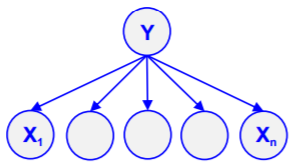
\includegraphics[height=0.3 \linewidth]{classification/pict/naivebayes.png}
	\caption{rete naive bayes}
\end{figure}

A fianco del risultato output comunque \`e bene fornire la probabilit\`a con il quale si \`e ottenuto il risultato, in modo da dare una \textit{misura di affidabilit\`a}. 

Il classificatore Naive bayes pu\`o essere applicato ad attributi categorici (nominali e ordinali), numerici (intervalli e tassi). Ogni attributo numerico è associato a una densit\`a di probabilit\`a condizionale di classe normale:

\[P(X_i = x_i | Y = y_k) = \frac{1}{\sigma_{ik}\sqrt{2 \cdot \pi}}exp(-\frac{(x_i-\mu_{ik})^2}{2 \sigma_{ik}^2})\] 

i cui parametri sono: \[\mu_{ik} = E[X_i | Y = y_k] \qquad \sigma_{ik}^2 = E[(X_i - \mu_{ik})^2 | Y = y_k]\]

\textbf{NB:} solitamente si combinano attributi categorici (nominali e ordinali) con attributi numerici (intervalli e tassi).

Naive bayes si comporta generalmente bene ma richiede \textit{\underline}{una enorme premessa} per essere applicato correttamente, (\textbf{indipendenza condizionata}). Quindi \`e stata creata una versione pi\`u flessibile mantenendo la stessa capacit\`a computazionale.

\subsubsection{Reti bayesiane}
Il classificatore Naive bayes \`e generalizzata dalla \textbf{Rete bayesiana} che \`e meno forzata dall'assunzione di indipendenza condizionata ma sfrutta il concetto di \textbf{Sparsity}. 

Un esempio di rete bayesiana è il seguente:

\begin{figure}[H]
	\centering
	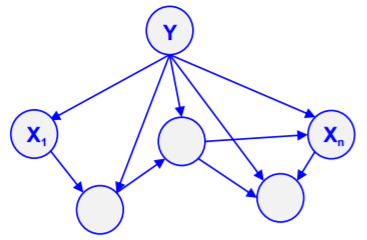
\includegraphics[height=0.35 \linewidth]{classification/pict/networkbayes.png}
	\caption{rete bayesiana generalizzata}
\end{figure}

Il nodo radice $Y$ che corrisponde all'attributo di classe.\\

Gli attributi esplicativi sono associati con i nodi, ma non solo quelli con un arco in entrata dalla radice, attributi esplicativi possono puntare ad altri attributi esplicativi.\\

Nel grafo \textbf{non} vi possono essere \textbf{cicli} in quanto un nodo successivo non pu\`o essere causa di un nodo precedente. Per ogni nodo va specificata una tabella di probabilità condizionata rispetto al valore dei suoi genitori. In sostanza prendo in considerazione tutte le possibili configurazioni dei genitori e per ognuna do un output diverso. \\

In questo modello gli attributi esplicativi non sono più assunti come indipententi dalla classe attributo.

Questo è un modello particolare di rete bayesiana che viene utilizzata per la classificazione. La cosa bella di questo modello \`e che anche con valori null si potrà comunque fare inferenza perchè nativamente ha questa caratteristica. \\

Al contrario, nelle reti neurali \textbf{non} \`e possibile far computare un modello senza che io abbia tutti gli input. 
\\
\subsubsection{Tree-augmented Naive Bayes}
Vi sono diverse versioni di reti bayesiane, una di queste è il Tree-augmented Naive Bayes.
\begin{defn}
\textbf{Tree-augmented Naive Bayes} oltre ad avere il nodo genitore Y pu\`o permettersi di avere un altro nodo genitore (sempre). Se io addestro la rete senza nodo di classe allora ho un albero, dopo inserendovi il nodo Y fa inferenza (nel caso in figura vedi nodo $X_1$).
\end{defn}

\begin{figure}[H]
	\centering
	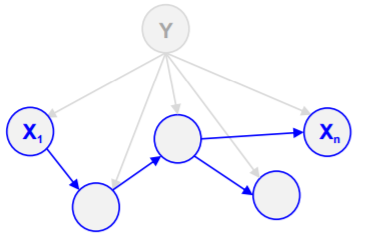
\includegraphics[height=0.35 \linewidth]{classification/pict/treenaivebayes.png}
	\caption{tree-augmented Naive bayes}
\end{figure}

\`E molto potente per la feature selection, ovvero per la ricerca delle feature pi\`u significative. 

Ci sono altre modifiche possibili al Tree-augmente naive bayes, presenti il letteratura, come AODE, HNB, ecc... 
\clearpage
\subsubsection{Summary}
Per capire come \textit{nativamente} si differenziano i modelli di classificazione vedi tabella successiva. 

\begin{figure}[H]
	\centering
	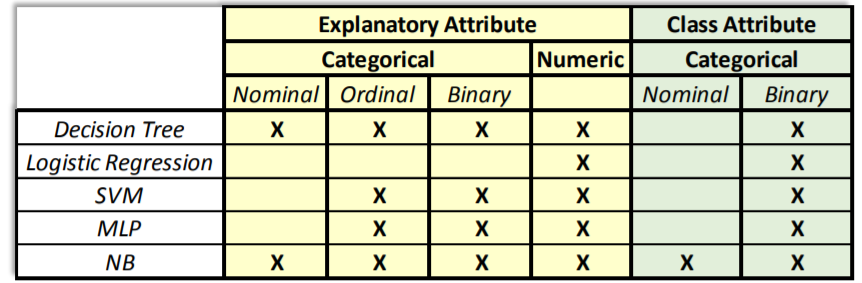
\includegraphics[height=0.3 \linewidth]{classification/pict/class_tecniques.png}
	\caption{comparazione tra i principali modelli nativi}
\end{figure}

In ogni caso, è possibile \textbf{trasformare} attributi esplicativi e di classe nominali applicando tecniche di classificazione non assegnate per attributi nominali. Notare comunque che le tecniche di classificazione \textbf{non} sono l'opzione migliore quando bisogna predire un attributo \textbf{ordinale}.

\subsection{Performance Evaluation (*)}
La stima dell'accuratezza non \`e sufficiente per comprendere la confidenza di un modello, in particolare quando bisogna applicarlo a dati mai visti.

Bisogna rendersi conto del rischio di \textbf{overfitting} quindi magnificare alcuni risultati, e di \textbf{underfitting} ovvero non abbastanza accurati.

Vi sono due diversi tipi di \underline{errori}:
\begin{itemize}
	\item \textbf{training error}: numero di record del training set mal classificato
	\item \textbf{generalization error}: errori non visti precedentemente nei record (test set)
\end{itemize}
Un buon classificatore non deve fittare troppo bene il training set ma deve anche classificare accuratamente i record che non ha mai visto prima (test set).\\

Inoltre sempre avere attenzione sulla qualit\`a dei dati, infatti considerare sempre il matra:
 
\textbf{Garbage IN Garbage OUT}\\

\begin{defn}
	Un modello di calssificazione che si allena su un training set troppo bene (basso training error) può avere un generalization error peggiore (stimato sul test set) rispetto ad un modello con alto training error, non va bene noi puntiamo a predire bene dati che non conosciamo. Si parla allora di \textbf{Overfitting del modello}.
\end{defn}

\underline{Nella pratica}: non devo adattare troppo il mio modello sui dati di training. 

Noi puntiamo ad un modello che "\textit{sbaglia}" (possibilmente poco) sia nel training set che nel test set in modo simile. Questa situazione significa che ho un modello che \textbf{non} ha overfittato. 

Consideriamo il seguente esempio
\begin{figure}[H]
	\centering
	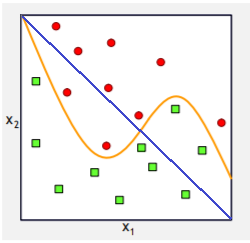
\includegraphics[height=0.3 \linewidth]{classification/pict/overfitting.png}
	\caption{esempio di overfitting}
\end{figure}
\begin{itemize}
	\item linea {\color{blue}{blu}}: modello con poco training error (non overfitting)
	\item linea {\color{orange}{arancione}}: modello con zero training error (overfitting)
\end{itemize}
Come si può notare il modello {\color{orange}{arancione}} si adatta troppo ai dati di training quindi c'è un forte rischio che non classifichi bene i dati di test. Al contrario il modello {\color{blue}{blu}} segue meglio la tendenza della distribuzione delle due classi di elementi.

Ora vediamo come si comportano i due modelli nel test set
\begin{figure}[H]
	\centering
	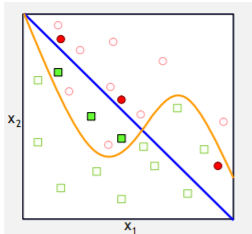
\includegraphics[height=0.3 \linewidth]{classification/pict/overfitting_test.png}
	\caption{esempio di overfitting test}
\end{figure}
Ora si può notare come il modello {\color{blue}{blu}}: più alto training error e più basso generalization error) classifichi \textbf{più correttamente} rispetto al modello {\color{orange}{arancione}}: più basso training error e più alto generalization error).

\begin{defn}
Il fenomeno contrario \`e l'\textbf{Underfitting}, in cui sia il training error che il generation error sono elevati. Accade quando performance del training e test sono simili e basse.
\end{defn}
La complessit\`a del modello scelto non \`e sufficiente per i dati che sto studiando. Non abbiamo utilizzato tutta la flessibilit\`a che potevamo usare nella definizione del modello.

\begin{figure}[H]
	\centering
	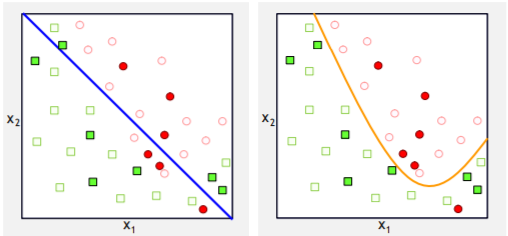
\includegraphics[height=0.3 \linewidth]{classification/pict/underfitting_merge.png}
	\caption{esempio di underfitting (sinistra)}
\end{figure}
Guardando agli esempi in figura, il modello {\color{blue}{blu}} classifica erroneamente 6 record, non è un buon modello. Invece, nel modello {\color{orange}{arancione}} fitta meglio il training ed risponde meglio anche al test (1 errore), in questo caso però bisogna stare attenti a non incappare in overfitting.\\
 
La \textbf{soluzione ottimale} la si evince da quello che succede nei dati di training e quello che succede nei dati di test.

\`E impossibile avere una misurazione certa sugli errori del modello, si pu\`o solo avere una stima. 

\subsubsection{Performance di un modello di classificazione}

In una analisi di classificazione vogliamo sviluppare un modello che ci dia una migliore classificazione possibile. Viene valutata in termini di:
\begin{itemize}
	\item Accuracy
	\item Speed
	\item Robustezza
	\item Scalabilit\`a
	\item Interpretabilit\`a (tema pi\`u dibattuto)
\end{itemize}

\subsubsection{Accuratezza}
L'accuratezza è una misura fondamentale perch\`e: 
\begin{itemize}
	\item misura la capacità del modello nel dare classificazioni affidabili su nuovi record
	\item ci permette di selezionare l'istanza di modello che d\`a le migliori performance sui nuovi record
\end{itemize}
Consideriamo:

$D_T$ training set con $t$ records

$D_{TS}$ test set con $v$ records

$D = D_T \cup D_{TS},D_T \cap D_{TS} = \emptyset,m = t + v$\\

Un buon indicatore è la percentale di record di test ($D_{TS}$) che sono classificati correttamente. 

Definiamo:
\begin{itemize}
	\item $y_i$ come il valore della variabile di classe dell'istanza $\underline{x_i} \in D_{TS}$
	\item $f(\underline{x_i})$ valore della classe predetto per l'istanza $\underline{x_i} \in D_{TS}$ dal modello di classificazione
\end{itemize} 
Consideriamo quindi la seguente funzione di loss:
\[
L(y_i, f(\underline{x_i})) =  
\begin{cases}
	0 \qquad se &y_i = f(\underline{x_i}) \\
	1 \qquad se &y_i \ne f(\underline{x_i})
\end{cases}
\]

l'\textbf{Accuratezza} viene calcolata in questo modo:
\[ acc(D_{TS}) = 1 - \frac{1}{v} \sum_{i=1}^{v} L(y_i, f(\underline{x_i}))\]

in alcuni casi si preferisce l'\textbf{Errore} associato:
\[err(D_{TS}) = 1 - acc(D_{TS}) = \frac{1}{v} \sum_{i=1}^{v} L(y_i, f(\underline{x_i}))\]

\subsubsection{Speed}
Gli algoritmi di classificazione differiscono per:
\begin{itemize}
	\item tempo di apprendimento
	\item spazio di memoria occupato
\end{itemize}
Oggi per\`o si da meno importanza a queste caratteristiche in quanto vi sono diverse tecnologie e tecniche ottimizzare i tempi e lo spazio di memoria costa sempre meno (economicamente parlando).

Un algoritmo che impega molto tempo e\o una grande quantità di memoria per l'addestramento, pu\`o essere trainato dopo un campionamento del dataset originale. In questi casi accettiamo di non sfruttare tutte le informazioni disponibili invece di trainare un tipo di modello che riteniamo assicurerà buone performance.

\subsubsection{Robustezza, Scalabilità e Interpretabilità}
\begin{defn}
	Un modello/algoritmo può essere \textbf{robusto} o meno rispetto a:
\begin{itemize}
	\item \underline{outliers}: possono influenzare significativamente il modello
	\item \underline{misssing data}: problema centrale (i dati di base sono sporchi e soggetti a deperimento)
	\item \underline{variazione tra training set e test set}: si parte dal presupposto che i dati di training siano simili e utili per quelli di test, se questa affermazione decade non \`e pi\`u robusto l'algoritmo
\end{itemize}
\end{defn}

\begin{defn}
	\textbf{Scalabilit\`a} \`e la capacit\`a di apprendere da enormi quantit\`a di dati. Questa proprietà è intresecamente connessa alla speed. 
\end{defn}
Es. le reti bayesiane scalano molto male. 

\begin{defn}
Quando la classificazione è orientata dall'\textbf{Interpretabilit\`a} di un problema per essere risolto e non ci si può limitare ad assicurare alti valori di accuratezza, è importante estrarre regole semplici e chiare per l'esperto di dominio del caso di studio.
\end{defn}
L'interpretabilit\`a \`e un problema enorme, perch\`e noi umani non ragioniamo in termini quantitativi, ma qualitativi. Una spiegazione pu\`o essere la pi\`u dettagliata e precisa possibile ma se non intercetta il linguaggio e il contesto in cui vive il soggetto che voglio raggiungere, non raggiungo il mio obiettivo di far interpretare il mio lavoro.

\subsubsection{Holdout}
\begin{defn}
L'\textbf{Holdout} è la partizione del dataset $D$ in due sottinsiemi di training e test set attraverso un procedura di campionamento. 
\end{defn}

\textbf{Best practice} suggerisce 2/3 per il training set e 1/3 per il test set.

Se si hanno molti dati a disposizione non \`e necessario seguire questa proporzione si pu\`o aumentare sul training.\\

\begin{figure}[H]
	\centering
	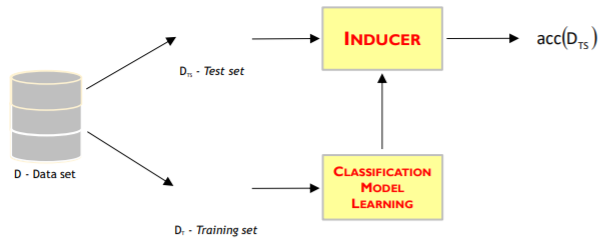
\includegraphics[height=0.3 \linewidth]{classification/pict/holdout.png}
	\caption{procedura di Holdout}
\end{figure}

La stima dell'accuratezza dipende dalla particolare scelta di divisione tra training e test set. Vi sono alcune tecniche per rendere più efficiente la divisione.

\begin{defn}
	\textbf{Iterated Holdout} consiste di ripetere iterativamente $R$ volte il metodo di holdout per cui apprendo e stimo l'accuratezza. 
\end{defn}
Ad ogni iterazione $r$ estraggo un campione random $D_{Tr}$ di $t$ records, e ottengo: 
	
$D_{TS_r} = D - D_{T_r}$
	
Ripeto la porcedura $R$ volte e l'accuratezza del classificatore è stimanata dalla media dei valori di accuratezza campionati $acc(D_{TS_r})$ calcolati su ogni test set $D_{TS_r}$:
	
\[ acc = \frac{1}{R} \sum_{r=1}^{R}acc(D_{TS_r})\]\\
	
Il numero di iterazioni $R$ può essere scelto tramite specifiche tecniche statistiche.

L'iterated Holdout è chiaramente un metodo pi\`u robusto, le sue performance hanno un bias più piccolo rispetto al normale holdout. Comunque, non permette il controllo del numero di volte in cui un record è presente nel training e test set. Non ho la certezza di aver usato dei dati ottimi per la stima fatta. In alcuni casi si ricorre a uno schema più efficace, capace di ridurre l'impatto degli outlier. 

\begin{defn}
	La tecnica di holdout detta	\textbf{Cross-validation} garantisce che ciascun record di un dataset $D$ sia incluso nel training set con lo stesso numero di volte e esattamente una volta nel test set. 
\end{defn}

Il dataset $D$ viene partizionato in $K$ sottoinsiemi disgiunti detti \textbf{fold}, esaustivi e con circa lo stesso numero di record: 

$D_1, D_2, ..., D_K$\\

Eseguiamo $K$ iterazioni training-test. Alla k-esima iterazione avremo:

$D_{T_k} = \{D_1, ...,D_{k-1},D_{k+1}, ...,D_K\} \qquad D_{TS_k} = D_k$

L'insieme $D_{T_k}$ è usato per il training  mentre il $D_K$ viene usato per il test della k-esima iterazione, in pratica ho più training set e un test set.

L'accuratezza viene stimata facendo la media delle $K$ iterazioni:

\[acc = \frac{1}{K} \sum_{k=1}^K acc(D_k)\]\\

che offre una stima più efficace dell'accuratezza del classificatore. \\

Esistono diverse selezioni per il valore di $K$. I valori tipici sono $K = 3,5,10$ mentre un caso limite viene applicato quando i dati sono scarsi chiamato \textbf{Leave One Out Cross Validation} (\textbf{LOOCV}). LOOCV è ottenuto assumento che ogni record è una partizione del dataset, così il valore di $K$ equivale al numero di record del dataset $D$.

\begin{figure}[H]
	\centering
	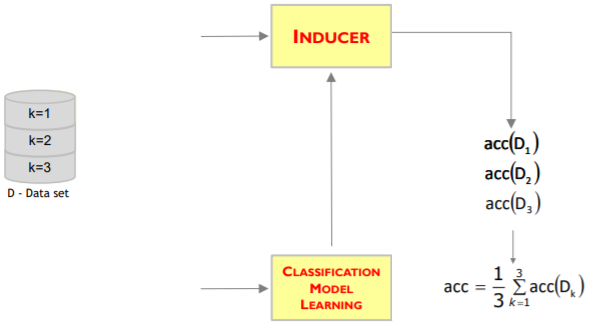
\includegraphics[height=0.3 \linewidth]{classification/pict/cross_validation.png}
	\caption{procedura di cross validation}
\end{figure}

Solitamente ci chiediamo se ogni partizione del dataset contiene la \textit{stessa proporzione} di valori possibili della classe attributo. Quando le proporzioni sono fortemente differenti si adottano specifiche tecniche di campionamento,es. \textbf{campionamento stratificato}. 

Noi in generale ci fidiamo di pi\`u del \textbf{k-folds cross-validation} in quanto rispetto all'\textit{iterated holdout} ho la certezza che i record non siano ripetuti.

\subsection{Comparing Classifiers (*)}
La comparazione tra due diversi \textit{classificatori} non è semplice, perchè dipende dai differenti modelli utilizzati e dalla distribuzione dei dati, nonchè la quantità. L'accuratezza ha diverso valore se ricavata da pochi record di dati. 
es. 
\begin{itemize}
	\item \textbf{Inducer A}: accuracy = 0.85 su un test set di 30 record
	\item \textbf{Inducer B}: accuracy = 0.75 su un test set di 5 000 record
\end{itemize}
Qual è il migliore?

L'accuratezza \textbf{non} basta. Bisogna stimare l'intervallo di confidenza dell'accuratezza per i due inducer e testare l'importanza statistica delle deviazioni osservate.
 
\subsubsection{Intervallo di confidenza}
Consideriamo il problema di predire il valore di una classe attributo da un test record come esperimento \textbf{binomiale}.

Dato un test set $D_N$ contenente $N$ record, consideriamo:
\begin{itemize}
	\item \textbf{X}: numero di record correttamente predetti dall'inducer
	\item \textbf{p}: vera, ma non la conosciuamo, accuratezza dell'inducer (probabilit\`a di successo della distribuzione binomiale)
\end{itemize}
Modelliamo il problema con X distribuita secondo una binomiale con
\begin{itemize}
	\item media = $N \cdot p$
	\item varianza = $N \cdot p \cdot (1-p)$
\end{itemize}
Oggetto del nostro studio \`e l'\textbf{accuratezza empirica}: \[acc = \frac{X}{N} \] 
che \`e distribuita secondo una binomiale con $\mu = p$ e $\sigma^2 = \frac{p \cdot (1-p)}{N}$

Sebbene la distribuzione binomiale possa essere usata per stimare l'intervallo di confidenza per l'accuratezza, se la dimensione del test set \`e sufficientemente grande, \`e buona norma approssimarla in una \textbf{normale}. Cos\`i facendo l'intervallo di confidenza per l'\textbf{accuratezza empirica} \`e:

\[ P \Bigl( -Z_{1-\alpha/2} < \frac{acc - p}{\sqrt{p \cdot (1-p / N)}} < Z_{1 - \alpha/2} \Bigr) = 1 - \alpha \]\\

Rimodellando la disuguaglianza ci porta al seguente intervallo di confidenza con confidenza $1-\alpha$ per \textbf{p}, la sconosciuta accuratezza del modello di classificazione:

\[ \Biggl[ \frac{acc + \frac{Z_{1-\frac{a}{2}}^2 }{2 \cdot N} - Z_{1-\frac{a}{2}} \cdot \sqrt{\frac{acc}{N} - \frac{acc^2}{N} + \frac{Z_{1-\frac{a}{2}}^2}{4 \cdot N^2}}}{\bigl(1 + \frac{Z_{1-\frac{a}{2}^2}}{N}\bigr)}
, 
\frac{acc + \frac{Z_{1-\frac{a}{2}}^2 }{2 \cdot N} + Z_{1-\frac{a}{2}} \cdot \sqrt{\frac{acc}{N} - \frac{acc^2}{N} + \frac{Z_{1-\frac{a}{2}}^2}{4 \cdot N^2}}}{\bigl(1 + \frac{Z_{1-\frac{a}{2}^2}}{N}\bigr)} \Biggr] \]\\
\underline{nota}: non chiede questa formula all'esame.

NB: se prendessi diversi test set indipendenti l'uno dall'altro \`e ovvio che vengono diversi intervalli di confidenza. Per\`o in questi casi fissato $\alpha$ posso stabilire statisticamente quali intervalli sono pi\`u significativi di altri. Pi\`u riduco $\alpha$ pi\`u aumenta $\beta$ ovvero il caso di errore in cui non rifiuto l'ipotesi nulla quando invece dovrei rifiutarla.

Dato un modello con acc=0.8 sul test set di $100$ record, fissiamo l'intervallo di confidenza per l'accuratezza a $0.95\%$. L'andamento dell'intervallo è il seguente:

\begin{figure}[H]
	\centering
	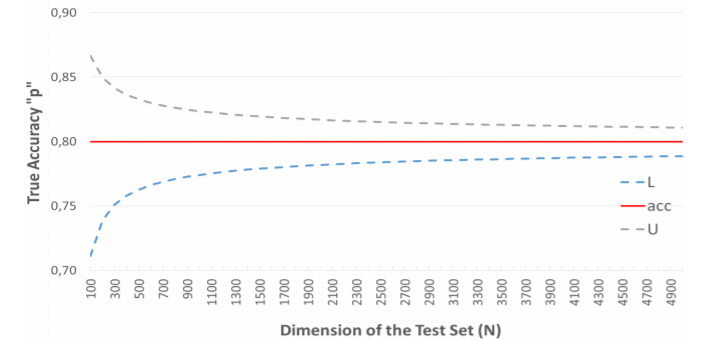
\includegraphics[height=0.5 \linewidth]{classification/pict/inter_confidence.png}
	\caption{esempio andamento dell'intervallo di confidenza}
\end{figure}

\subsubsection{Different test set}
Supponiamo il caso in cui ho 2 modelli e vengono valutati per forza su due test set diversi (per tanti motivi pu\`o succedere):
\begin{itemize}
	\item $M_1$ valutato su test set $D_1$ contenente $n_1$ record con tasso di errore $e_1$
	\item $M_2$ valutato su test set $D_2$ contenente $n_2$ record con tasso di errore $e_2$
\end{itemize}
I due test set devono essere assunti \textit{indipendenti}. Il nostro obiettivo \`e testare se la \textbf{differenza} tra i due errori \`e statisticamente significativa.

Assumiamo che $n_1$ e $n_2$ siano sufficientemente grandi, allora i tassi di errore $e_1$ ed $e_2$ possono essere approssimati usando distribuzioni \textit{normali}.

La differenza osservata \`e denotata come: 
\[d = e_1 - e_2\]
sono distribuiti secondo una \textbf{normale} con 
\[\mu = d_t \qquad \sigma^2 = \sigma^2_d\] 

La varianza di d pu\`o essere stimanata come segue: 
\[\sigma^2 \cong \hat{\sigma}_d^2 = \frac{e_1 \cdot (1-e_1)}{n_1} + \frac{e_2 \cdot (1-e_2)}{n_2}\]

L'intervallo di confidenza per la differenza $d_t$ \`e: 

\[ \bigl( d - z_{1-\alpha/2} \cdot \hat{\sigma}_d, d + z_{1-\alpha/2} \cdot \hat{\sigma}_d \bigr) \]

Ci possono essere sostanzialmente 3 casi:
\begin{enumerate}
	\item \[0 \in \bigl( d - z_{1-\alpha/2} \cdot \hat{\sigma}_d, d + z_{1-\alpha/2} \cdot \hat{\sigma}_d \bigr)\] allora concludiamo che la differenza osservata \textbf{non \`e statisticamente significativa} ad un livello $\alpha$, i modelli non sono significativamente differenti 
	\item \[d + z_{1-\alpha/2} \cdot \hat{\sigma}_d < 0\] se il limite superiore della confidenza \`e negativo allora il modello \textbf{$M_1$ \`e migliore del modello $M_2$} a un livello $\alpha/2$
	\item \[d - z_{1-\alpha/2} \cdot \hat{\sigma}_d > 0\] se il limite superiore della confidenza \`e positivo allora il modello \textbf{$M_2$ \`e migliore del modello $M_1$} a un livello $\alpha/2$
\end{enumerate}

Buona norma fare il test di ipotesi \textbf{solo} se prima mi faccio la domanda se sono o meno differenti, non continuare a condurre test a casaccio o a tappeto perch\`e altrimenti si rischia di raggiungere degli assurdi. Bisogna farsi la domanda e poi eseguire tutta la procedura sulla coppia di modelli, in quanto vi \`e un \textbf{problema dei confronti multipli} devo adattarli tutti allo stesso livello di $\alpha$ altrimenti non sono confrontabili le differenze. \\

\subsubsection{Same test set}
Nel caso in cui ho lo \textbf{stesso test set} posso svolgere un test pi\`u \textbf{potente} ovvero posso valutare il caso di errore di secondo tipo: affermo che la differenza tra i due classificatori non \`e significativa quando in realt\`a lo \`e ($\beta$). 

Si confrontano $M_1$ ed $M_2$ usando il \textit{k-fold cross validation}.

Ho il dataset $D$ partizionato in $K$ subset disgiunti con circa lo stesso numero di record. 
\[D_1, D_2, ..., D_K\]

Applichiamo le tecniche di classificazione per costruire i modelli $M_1$ e $M_2$ dalle $k-1$ partizioni e li testiamo con la partizione rimanente. Il passaggio deve essere ripetuto $K$ volte, ogni voltausando una differente partizione per il test set. Ottengo:
\begin{itemize}
	\item $M_{1k}$ \textbf{inducer} per il modello $M_1$ ottenuto alla k-esima iterazione con $e_{1k}$ errore
	\item $M_{2k}$ \textbf{inducer} per il modello $M_2$ ottenuto alla k-esima iterazione con $e_{2k}$ errore
\end{itemize}

La differenza tra gli errori durante la k-esima iterazione è:
\[d_k = e_{1k} - e_{2k}\]
Per K sufficientemente grande, allora $d_k$ \`e distribuito \textit{normalmente} con: 
\[\mu = d_t^{cv} \quad \sigma = \sigma^{cv}\]

dove la varianza osservata \`e stimata secondo la seguente formula: 

\[ \hat{\sigma}^2_{d^{cv}} = \frac{\sum_{k=1}^{K}(d_k - \bar{d})^2}{K \cdot (K-1)} \qquad \bar{d} = \frac{1}{K} \sum_{k=1}^K d_k \]

Usiamo una distribuzione T di Student per calcolare l'intervallo di confidenza per il valore della vera media $d_t^{cv}$

\[\biggl( \hat{d} - t_{1-\frac{\alpha}{2}}^{K-1} \cdot \hat{\sigma}_{d^{cv}}
,
\hat{d} + t_{1-\frac{\alpha}{2}}^{K-1} \cdot \hat{\sigma}_{d^{cv}} \biggr)\]

dove 
\[t_{1-\frac{\alpha}{2}}^{K-1}\]

è ottenuta dalla tavola di probabilità, il quantile associato alla confidenza $1-\alpha$ e $K-1$ gradi di libertà.\\

Ovviamente valgono \textbf{le stesse condierazioni} fatte precedentemente sull'intervallo di confidenza fatte precedentemente per la differenza tra due classificatori. 

Se l'intervallo di confidenza contiene il valore 0, concludiamo che la differenza osservata \textit{non è statisticamente significativa} al livello $\alpha$ (confidenza $1-\alpha$). 

\subsection{Class Imbalance Problem (*)}
Consideriamo di nuovo il dataset dei Churner. In particolare sappiamo che il $14.5\%$ sono dei churner. Un modello di classificazione che etichetta i record come non churner avrà per forza un'alta accuracy in quanto è la classe più frequente nel dataset. 

\begin{defn}
	Il modello più inutile è quello che risponde sempre con la classe più frequente, ovvero la \textbf{ZeroR Rule}.	
\end{defn}
\begin{comment}
Bisogna studiare la classe pi\`u rara (meno frequente), essa viene denotata come \textbf{classe positiva}, mentre quella pi\`u frequente \`e detta \textbf{classe negativa}.

Consideriamo la \textbf{matrice di confusione}, allora possiamo calcolare:
\begin{itemize}
	\item specificit\`a (tasso veri negativi) $TNR = \frac{TN}{TN + FP}$
	\item sensitivit\`a (tasso veri positivi) $TPR = \frac{TP}{TP + FN}$
	\item tasso falsi positivi $FPR = \frac{FP}{TN + FP}$
	\item tasso falsi negativi $TNR = \frac{FN}{TP + FN}$
\end{itemize}

Viene definito un indice chiamato \textbf{precisione}: $p = \frac{TP}{TP+FP}$, ovvero il punto di vista del classificatore. Valuto quanti di quelli positivi ha valutato come effettivamente positivi. 

Viene anche definito il \textbf{recall} (richiamo): $r = \frac{TP}{TP+FN}$, in questo caso ho il punto di vista della realt\`a. Sotto ho quelli effettivamente positivi, sopra ho quelli che il classificatore ritiene positivi. \`E la capacit\`a del classificatore di richiamare i risultati positivi (quanti dei positivi \`e riuscito ad aspirare?). 

Vi \`e un legame molto stretto tra questi due indici, posso avere una recall molto alta ma allora probabilmente avrò una precisione bassa. Oppure potrò puntare ad avere una precisione alta ma in quei casi probabilmente avrò una recall bassa.

\underline{NB} queste due misure per convenzione sono calcolate sulla classe positiva (quella pi\`u frequente) non \`e per\`o detto che non vadano utilizzate su quella negativa. Inoltre non \`e sempre detto che queste quantit\`a siano sempre calcolabili (vedi es. slide).

Siccome queste due misure sono legate (pensa alla coperta corta). Si utilizza una misura che le riassume chiamata $F_1$ measure:

\[ F_1 = \frac{2 \cdot r \cdot p}{r + p}\]

$F_1$ \`e una misura media armonica tra recall e precision. Un alto valore di $F_1$ implica alti valori di recall e precision.

Generalizzazione:

\[ F_\beta = \frac{(\beta^2 + 1) \cdot r \cdot p}{r + \beta^2 \cdot p} \]

\begin{itemize}
	\item $F_\beta$ con $\beta = 0$ \`e la Precisione
	\item $F_\beta$ con $\beta = \infty$ \`e la Precisione	
\end{itemize}

\section{Lezione 8}

\subsection{Matrice di costo}
Se pensiamo al nostro problema del churner, l'azienda ha interesse ad evitare quello che si prevede, ovvero che il cliente se ne vada, in sostanza cerco di prevedere chi vuole andarsene e cerco di evitare che questa previsione sia effettiva. L'azienda pu\`o spendere un tot budget per invertire questo fenomeno, devo fare il meglio per identificare i possibili churner e attuare SOLO su di loro le politiche di dissuasione (se lo facessi per tutti i clienti non avrebbe senso per quanto riguarda i costi).

Bisogna convincere il proprio interlocutore che il modello da me sviluppato sia migliore rispetto al modello che storicamente hanno utilizzato. Con l'accouracy \`e facile. Bisogna associarci la \textbf{matrice di costo} che stabilisce in base a falsi positivi e negativi quanto costo (in soldi) sostiene l'azienda in base alla situazione. 

Costo: $Cost = C_{--} \cdot TN + C_{-+} \cdot FP + C_{+-} \cdot FN + C_{++} \cdot TP$

\textbf{NB} se matrice di costo \`e simmetrica allora il costo corrisponde all'accuratezza.

\begin{figure}[h!]
	\centering
	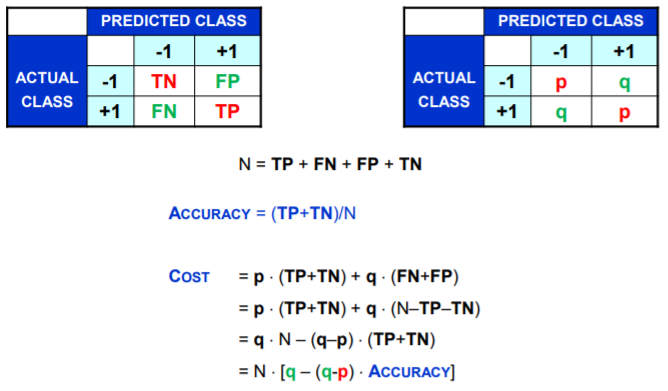
\includegraphics[height=0.55 \linewidth]{classification/pict/matr_costo.png}
	\caption{legame tra matrice di confusione (sn) e matrice di costo (dx)}
\end{figure}

\subsection{Cumulative Gains}
\`E importante notare per\`o che ci sono situazioni nelle quali perdere un cliente \`e pi\`u grave che perderne un'altro. Devo capire se sto utilizzando la matrice dei costi vera oppure se \`e solo rappresentativa. Se essa non \`e certa posso ragionare in un altro modo. 

Supponiamo che suddividiamo la nostra popolazione in campioni casuali. Vengono valutati la zero rule (campionamento casuale) il modello storico dell'azienda e il nostro modello di classificazione. Si verifica che in termini percentuali il nostro modello fa 60\% e il campionamento casuale fa 37.5\%. 
Il \textbf{List Factor} = rapporto tra i due modelli. 

\textbf{NB}: considera che il nostro classificatore \`e bravo ad identificare i casi semplici ma rischia di sbagliare di molto in quelli complessi. Man mano che lo forzo a rispondere lui risponder\`a in modo sempre pi\`u random

Per comprendere il \textit{livello di profittabilit\`a} pu\`o essere calcolate una volta che si conoscono i costi coinvolti. Nel nostro caso vogliamo:
\begin{itemize}
	\item alta proporzione di record positivi
	\item alto numero di elementi del set
\end{itemize}

Se ordinassi gli output con probabilit\`a di riconoscimento corretto in ordine decrescente. Posso calcolare il List Factor sui primi risultati per comprendere fino a dove ha buone performance. Man mano aumento gli elementi di risultato per comprendere la sua efficacia se considero elemento con probabilit\`a minore. Quanto ha senso considerare output con bassa probabilit\`a per valutare il mio modello?

Viene quindi visualizzata la cosiddetta curva del \textbf{cumulative gains} ovvero la curva che evidenzia questo fenomeno.
\begin{figure}[h!]
	\centering
	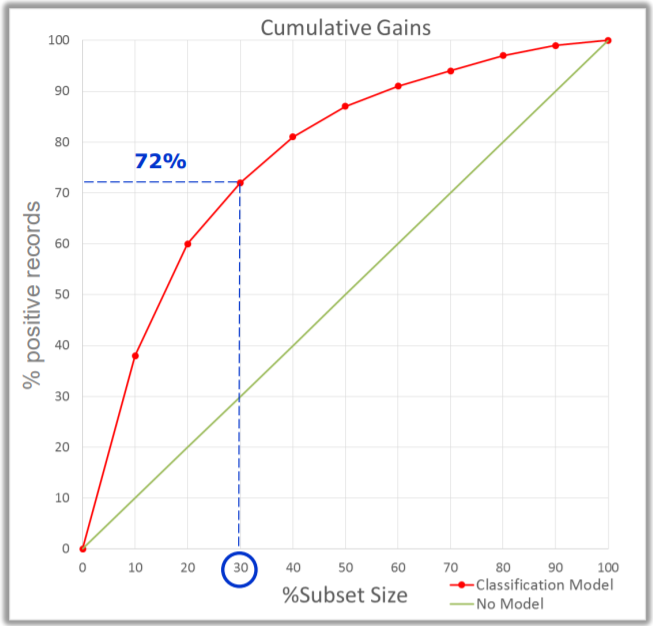
\includegraphics[height=0.6 \linewidth]{classification/pict/cumulative_gains.png}
	\caption{cumulative gains evidenziando un punto di alto valore aggiunto}
\end{figure}

NB: la retta verde calcola la cumulative gain per un modello che risponde in maniera casuale, sull'asse x \`e la recall, i positivi riconosciuti correttamente (ricordati ripetendo il test non per un caso ad ogni percentuale)

\subsection{Lift Chart}
La curva di lift chart \`e derivata direttamente dalla mappatura della cumulative gains.

\begin{figure}[h!]
	\centering
	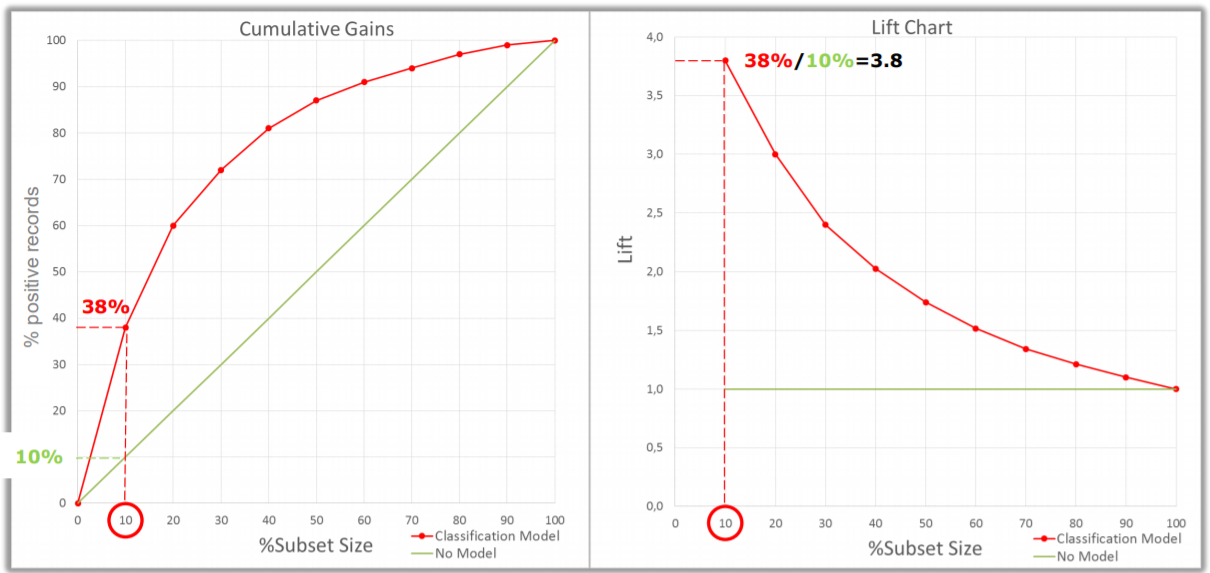
\includegraphics[height=0.45 \linewidth]{classification/pict/lift_chart.png}
	\caption{da cumulative gain a lift chart}
\end{figure}

Queste valutazioni ci fanno comprendere quando il nostro classificatore perde efficacia. Naturalmente pi\`u il campione \`e piccolo meglio funziona, bisogna comprendere per\`o il punto di massima accuratezza in rapporto alla percentuale di istanze.

\subsection{Curva ROC}
Assomiglia molto alla cumulative gains ma sull'asse delle x ho la percentuale di falsi positivi sopportabili, e sulle y i veri positivi corrisposti. \`E chiamata \textbf{ROC} e sta per Receiver Operating Characteristic curve. 
\begin{figure}[h!]
	\centering
	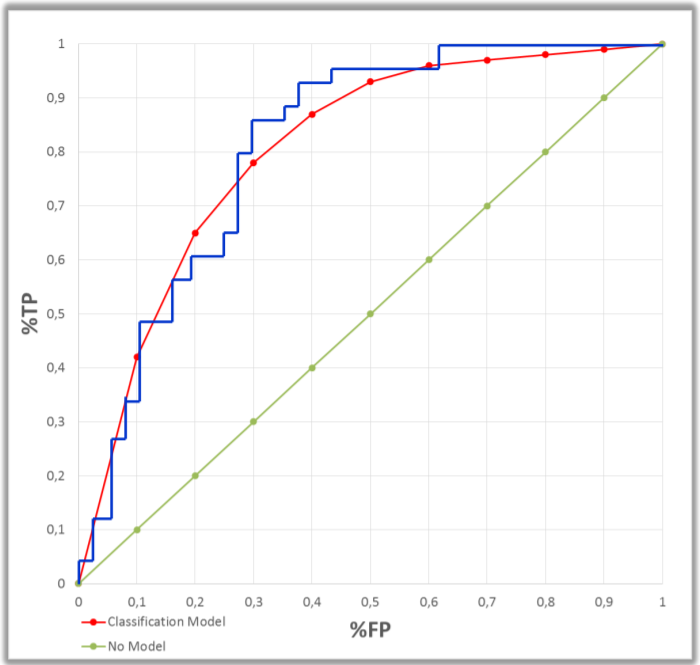
\includegraphics[height=0.6 \linewidth]{classification/pict/roc.png}
	\caption{curva ROC legata a dataset variabili (pi\`u reale)}
\end{figure}
Serve a confrontare diversi classificatori per cercare di comprendere dove un classificatore \`e pi\`u o meno efficace. 

Un modello \`e preferibile ad un altro se \`e disposto a sopportare un certo numero di falsi positivi e valuto quanto veri positivi ci sono. 

\begin{figure}[h!]
	\centering
	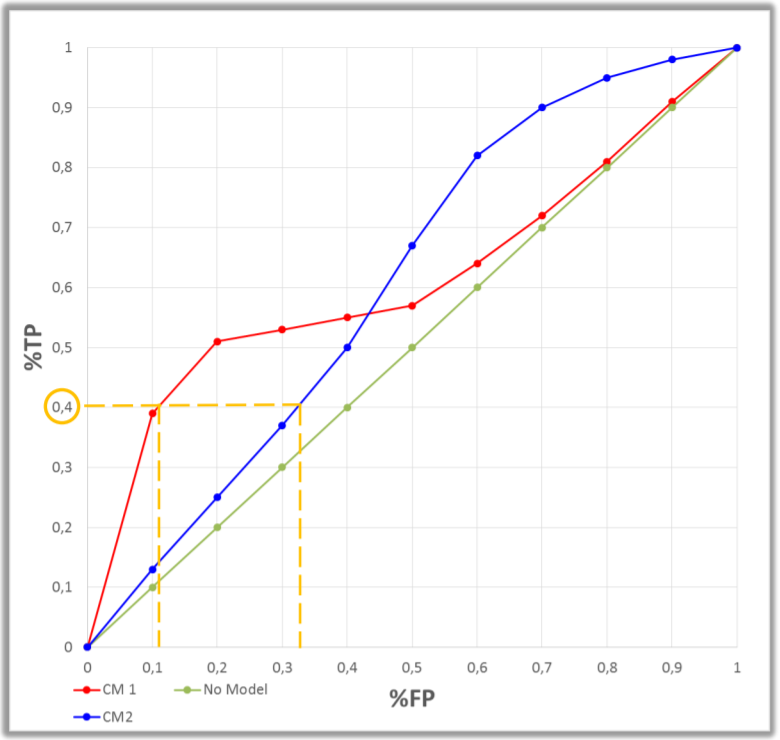
\includegraphics[height=0.6 \linewidth]{classification/pict/roc_confronto.png}
	\caption{confronto ROC da due modelli}
\end{figure}
\clearpage
\section{Lezione 9 - Feature Selection}
La feature selection \`e un compito importantissimo ed \`e legato gi\`a alla risoluzione del problema. Analizzare le relazioni tra le variabili in modo preliminare potrebbe gi\`a aiutare di molto nella ricerca della soluzione migliore al problema. 

Quasi sempre non ha senso utilizzare tutti gli attributi per generare il modello che si vuole sviluppare. Quindi si procede con la selezione delle feature.
\begin{itemize}
	\item attributi \textbf{ridondanti} ovvero quelli dei quali l'informazione \`e gi\`a contenuta in altri attributi. La rilevanza va sempre valutata in base ai dati a disposizione
	\item attributi \textbf{irrilevanti} contengono informazioni non utili per risolvere il problema di data mining.
\end{itemize}
Vi sono diversi approcci per rilevare questi attributi:
\begin{itemize}
	\item \textbf{Brute-force}: provo tutti i modelli per ogni combinazione di parametri usati nel modello di Classificazione. Ma la computazione di questi casi \`e troppo grossa, vi sono: $\sum_{n=1}^{10}\left(10 n\right)$ possibili combinazioni
	\item \textbf{Embedded}: attributi scelto in base alla capacit\`a di fare split della classificazione (pensa agli alberi di decisione)
	\item \textbf{Filter}: attributi selezionati pima del classificatore in base a quelli che si ritengono pi\`u rilevanti e meno rilevanti (analisi di funzione obiettivo)
	\item \textbf{Wrapper}: gli attributi che si scelgono in base al modello di classificazione scelto, quelli che sono rilevanti per un modello non lo sono per un altro (dipende dall'ipotesi che ho fatto)
\end{itemize}
\begin{figure}[h!]
	\centering
	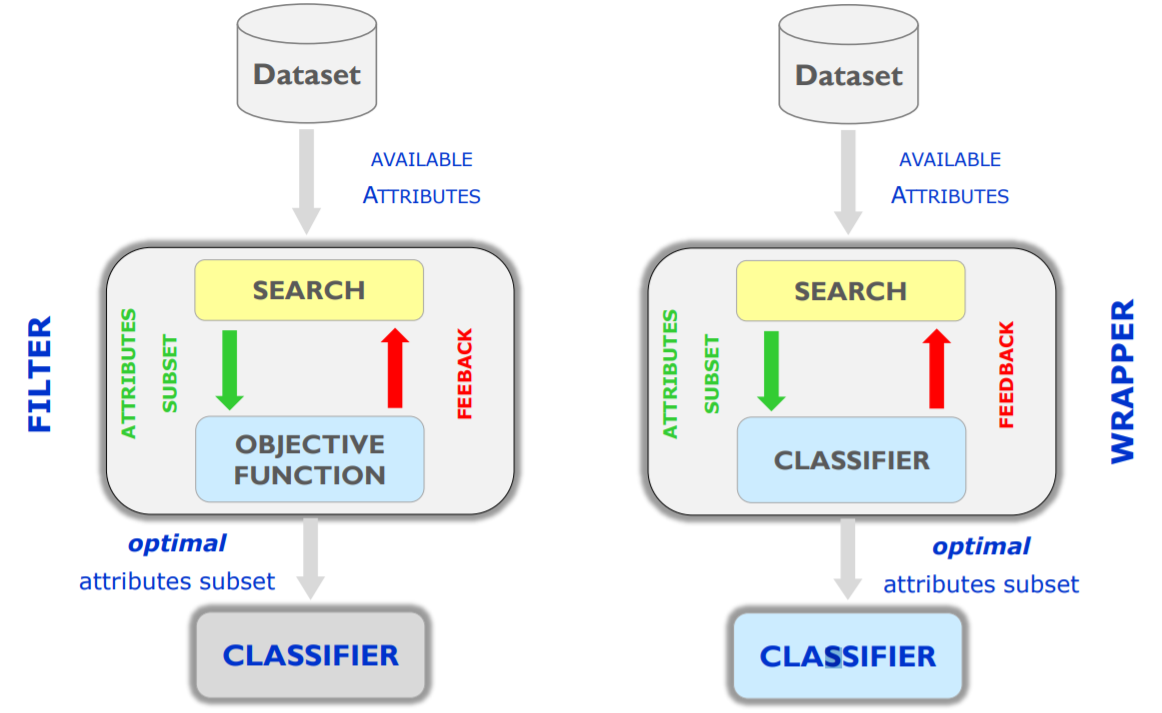
\includegraphics[height=0.45 \linewidth]{classification/pict/filter_wrapper.png}
	\caption{Filter - Wrapper, due differenti approcci per feature selection}
\end{figure}
\textbf{NB} non va bene fare feature selection su tutti i dati e poi trainare solo su un sottoinsieme!! altrimenti si hanno risultati non comparabili
\\
\textbf{Filter} nel caso di attributi \textit{uni-variati}: 
\begin{enumerate}
	\item si scegle una misura di associazione tra gli attributi candidato e quello di classe
	\item si ordinano gli attributi in base alla misura di associazione
	\item si selezionano le prime $R$ posizioni come attributi di input per il classificatore
\end{enumerate}
solitamente si identificano gli attributi irrilevanti, per\`o non funziona bene nella ricerca di attributi ridondanti.

multi-variati:
\begin{itemize}
	\item identificano insieme attributi rilevanti e irrilevanti
	\item un buon sottoinsieme di attributi deve contenere attributi fortemente associati con l'attributo di classe ma essere incorrelati tra di loro
\end{itemize}

\begin{figure}[h!]
	\centering
	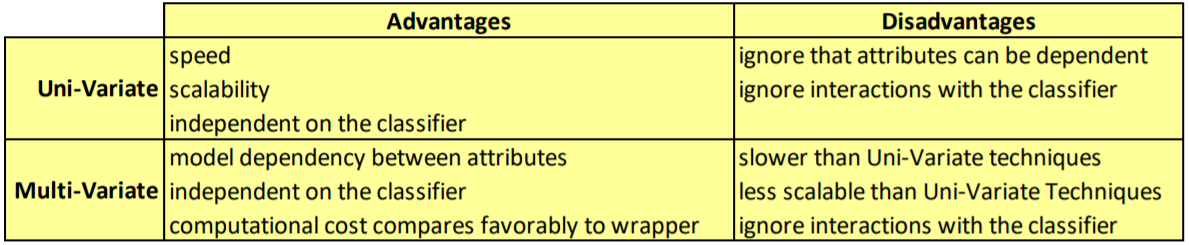
\includegraphics[height=0.22 \linewidth]{classification/pict/filter_uni_multi.png}
	\caption{vantaggi e svantaggi tra tecniche uni-variate e multi-variate}
\end{figure}

Vantaggi pe la feature selection sono:
\begin{itemize}
	\item riduzione del costo di collezione di dati
	\item riduzione dei tempi di inferenza del classificatore relativo all'attributo di classe
	\item pi\`u alta interpretabilit\`a
	\item aumento dell'accuratezza
\end{itemize}
Motivazioni:
\begin{itemize}
	\item evitare l'overfitting
	\item sviluppo di un miglior cost-effective classifier
	\item migliorare la comprensione del processo di generazione dati
\end{itemize}

Flowchart da seguire:
\begin{figure}[h!]
	\centering
	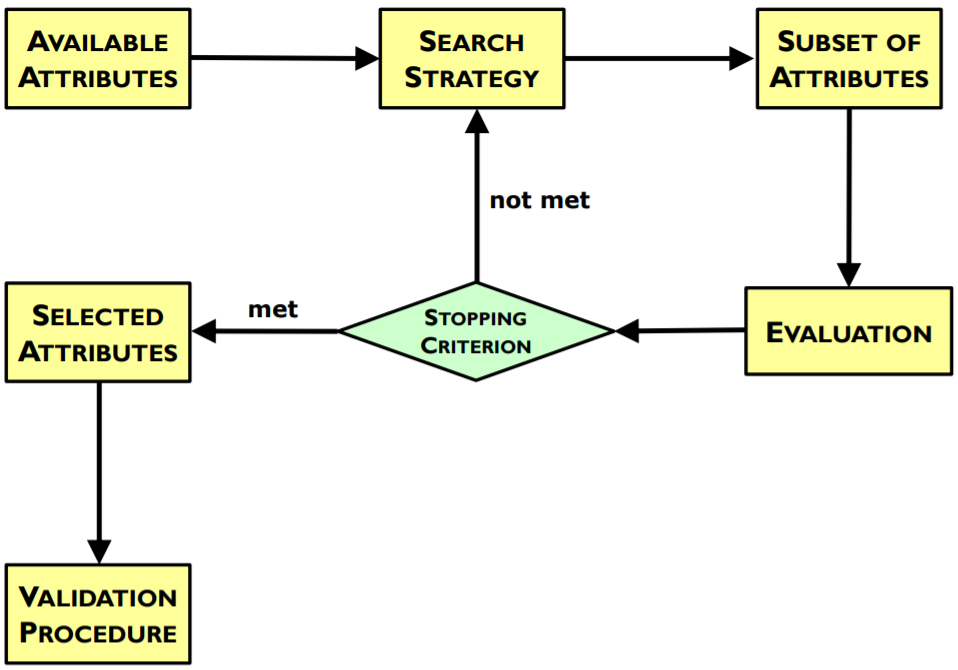
\includegraphics[height=0.45 \linewidth]{classification/pict/feature_flowchart.png}
	\caption{vantaggi e svantaggi tra tecniche uni-variate e multi-variate}
\end{figure}
\\
La creazione di nuove feature dai dati:
\begin{itemize}
	\item feature extraction: utilizzati per classificazione di immagini/segnali
	\item mappare dati in un uovo spazio: vedere gli attributi in modo normalizzato o secondo un'altra scala pi\`u facilmente trattabile (SVM)
	\item feature construction: generare feature nuove pi\`u comode per un certo modello di classificatore rispetto a quelle originali attrivarso trasformazioni, es. logaritmi di somme ecc.. (non \`e detto che i dati originali siano i pi\`u utili per la classificazione)
\end{itemize}

\section{Lezione 10 - Classificazione NON binaria}

Nei problemi reali la classificazione avviene su pi\`u valori non solo binari.

L'idea \`e quella di trasformare un problema multi-classe in tanti attributi di classe binari. \textbf{Multi-classe} esattamente una classe si realizza. \textbf{Multi-etichetta} pi\`u di una classe pu\`o verificarsi. Vi possono essere anche problemi non di classe ma di \textbf{ranking} in cui i valori assunti dalla variabile di classe sono ordinati.

\subsection{One-Vs-All}
In questa modalit\`a si verifica se il set corrente verifica o meno ciascuna delle caratteristiche da valutare. 

Ricorda che non sempre binarizzare \`e necessario, in particolare per quanto riguarda i naive bayes non serve, invece per un decition tree s\`i. 

Nel \textit{One-vs-all} creo un numero di classificatori diverso in base al numero di modalit\`a dell'attributo di classe. Inoltre bisogna normalizzare poi gli output dei classificatori. Nel modello \textit{multi-label} bisogna prendere i valori cos\`i come li restituisce il cassificatore e fissare un threshold sopra il quale considero signficiativo il risultato (potenzialmente pi\`u di una classe supera il threshold). 

\subsection{Train/validation/test e feature selection}
Una rete neurale \`e dimostrato che permette architetturarla per approssimare qualsiasi problema. Non \`e per\`o esente da overfitting anzi visto che non \`e sempre chiaro il funzionamento \`e pi\`u difficile valutarle. 

Se volessimo scegliere i parametri (pesi e soglie) e un \textbf{iperparametro} $\lambda$ detto di \textit{regolarizzazione}. Voglio sceglere qella allocazione di parametri per ridurre il pi\`o possibile l'errore quadratico del modello, quindi l'iperparametro. 

\[ E(w, \lambda) = \frac{1}{m} \sum_{i=1}^{m}(y_i \hat{y}_i)^2 + \frac{\lambda}{2} \sum_{j=1}^{K} w_i^2 \]

La prima parte \`e il fitting della funzione, la seconda parte \`e la flessibilit\`a alla quale posso accedere. Potenzialmente io posso imparare il valore ottimale di $\lambda$ dai dati. 

Per questo suddivido il dataset in train e test. Se utilizzazzi i dati di training per imparare il migliore lambda allora andrei in overfitting di lambda. Quindi suddivido in questo modo il dataset:
\begin{itemize}
	\item train dataset viene utilizzato per trainare il modello (sui parametri w)
	\item validation dataset che viene utilizzato per trainare su lambra
	\item test dataset viene utilizzato per testare definitivamente il modello
\end{itemize} 

\textbf{NB} se utilizzo il test set per ottimizzare il parametro lambda allora ho bruciato il dataset e devo rifare, obiettivo \`e sempre quelo di riconoscere dati mai visti.
\end{comment}